\documentclass[11pt]{article}
\usepackage[margin=1in]{geometry}
\usepackage{amsmath}
\usepackage{graphicx}
\usepackage{tikz-cd}
\usepackage{multicol}
\usepackage{array}
\usepackage{tabularx}
\usepackage{url}

\setlength{\parindent}{0pt}
\setlength{\parskip}{1\baselineskip}

\title{The EYES Manual}
\author{Zifei Zhong\\(draft 2)}

\begin{document}
\maketitle
\tableofcontents

\newpage
\section{Design Purpose}
The EYES toolbox is designed to process and analyze log files collected from Android smart devices (phones and tablets) by the App Chronicle. The toolbox generates outputs such as App Usage, Device Pickups, Visualization, and integrated event timelines. The toolbox can be launched either from the command line or from a desktop GUI, where a user selects a folder containing raw Chronicle \texttt{.csv} files and runs the full pipeline with one click.

\section{Data Characteristics of the Chronicle Log Files}
The Chronicle log files are collected on a user device and then uploaded to a server. Some characteristics that we have observed in the data include:
\begin{enumerate}
\item Missing data: Some event logs might not be uploaded to the server successfully, thus causing missing data. For example, there may be a `Screen Interactive' event in the log file, but the corresponding `Screen Non-interactive' event is missing.
\item Duplication: Some event logs are uploaded multiple times, thus causing duplicated rows in the same file.
\item Out-of-order rows: In general, the log file records rows in increasing time order based on `event\_timestamp'. However, this is not always true. Many files contain rows recorded out of order.
\end{enumerate}

There might be other issues that we are not aware of. We will keep the document updated when we have new observations.

 \subsection{Data File Format}
 The EYES toolbox takes raw data files as input. The raw data files are `.csv' files in which each row logs an event, including information such as `app\_package\_name', `interaction\_type', and `event\_timestamp'. Figure~\ref{fig:raw-data} shows the raw data file format.

One recommended practice is to put all raw files in one directory and provide the path to this directory to the EYES toolbox. Then all raw data files in that directory will be processed.

\begin{figure}[ht]
  \centering
  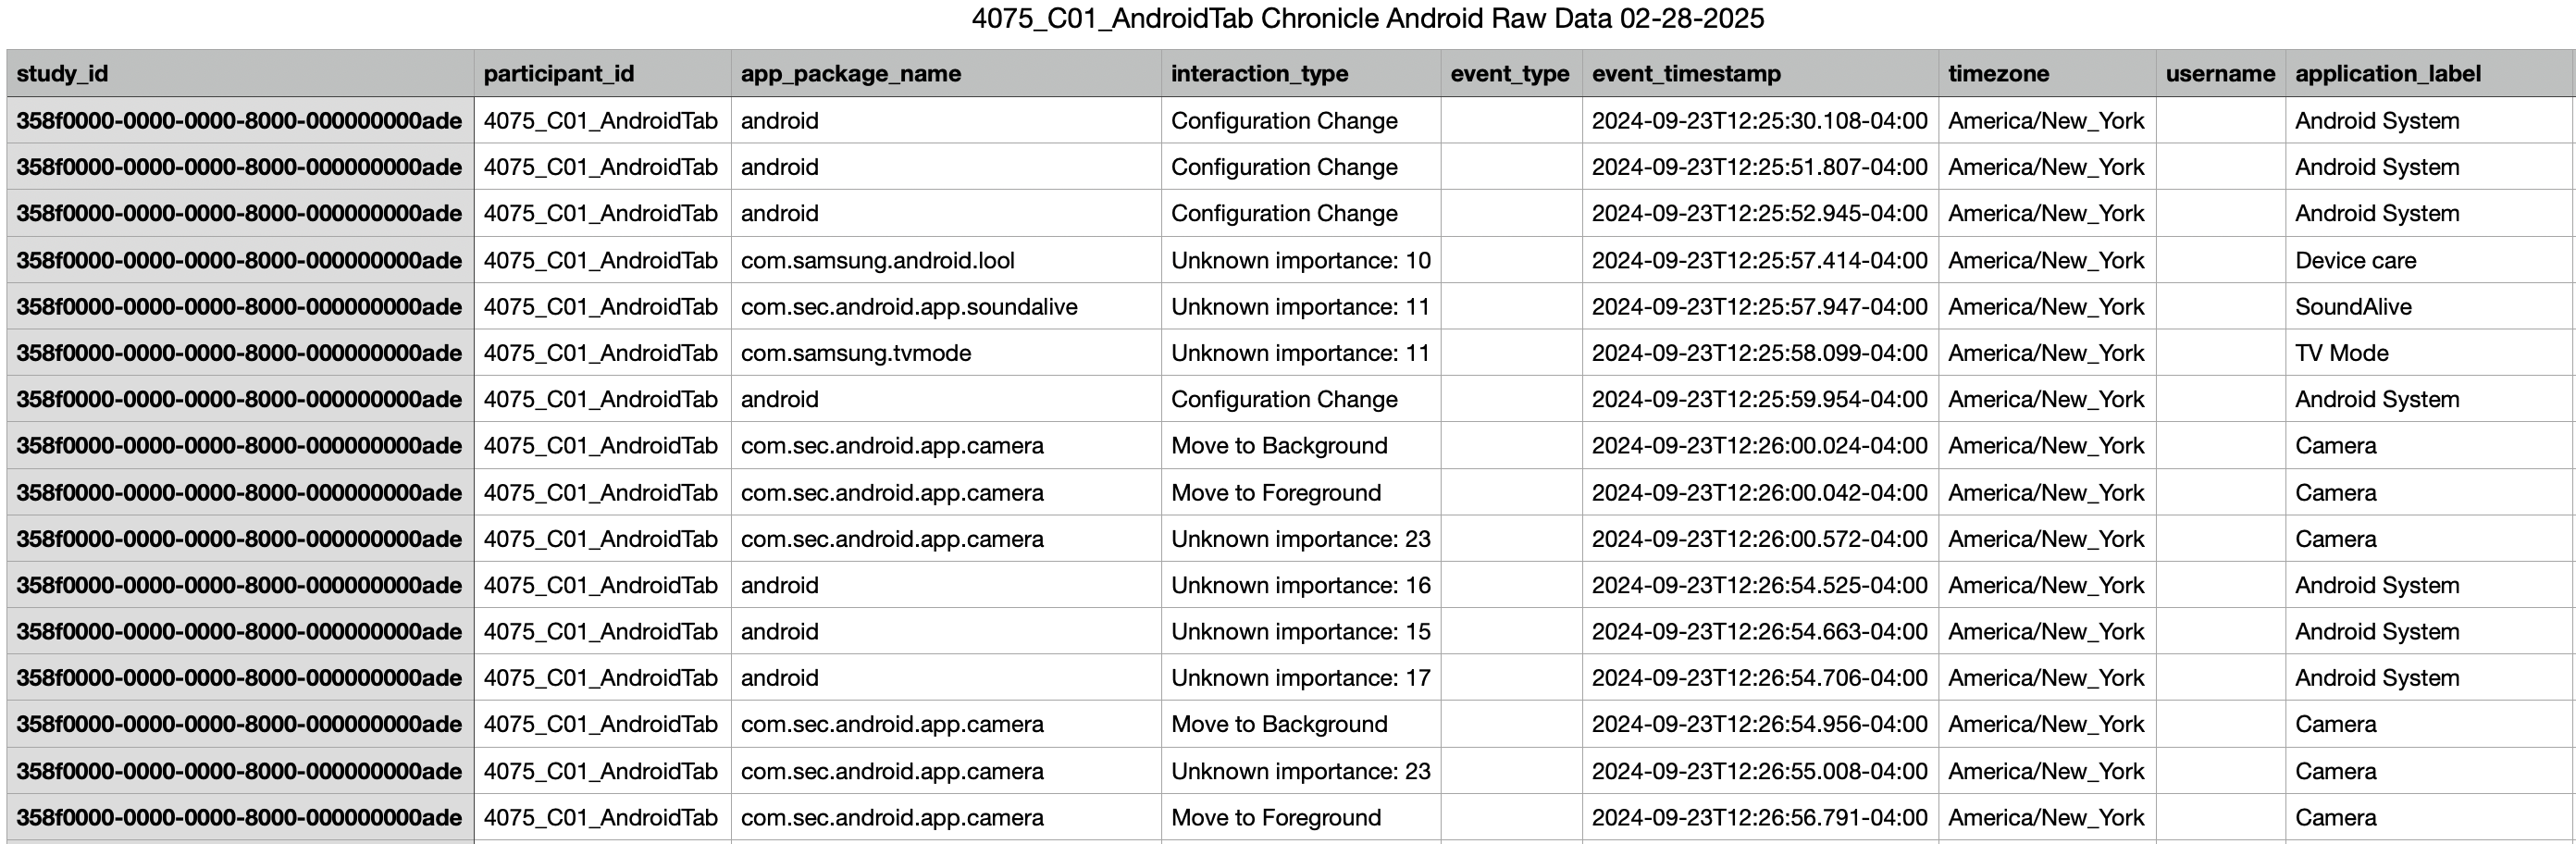
\includegraphics[width=0.75\textwidth]{imgs/raw-data.png}
  \caption{Raw data file format.}
  \label{fig:raw-data}
\end{figure}

\section{Design Philosophy}
The EYES toolbox analyzes the log data by:
\begin{itemize}
\item Identifying the internal states of the device: ACTIVE, GLANCE, IDLE, SHUTDOWN, GAP.
\item Constructing the logic structure of an activity (triplet): Activity Resumed, Activity Paused, Activity Stopped.
\item Inference: A set of inference rules is programmed into the toolbox scripts to ensure detailed analysis. For example, if no `Activity Stopped' event exists, then the toolbox uses the pair (`Activity Resumed', `Activity Paused') as the app usage interval; if only `Activity Resumed' exists, then it uses the next app's `Activity Resumed' event as the termination of the previous app usage interval.
\item Combining the above to accurately extract App usage or device pickups.
\end{itemize}

Other data analysis tools also exist. For example, the Uzair (cite) scripts are widely used. However, the data processing logic of the Uzair tool is very different from that of the EYES toolbox. The Uzair tool simply matches each `Activity Resumed' event to the next available `Activity Paused' event and uses that interval as app usage. While this works for common app activity scenarios, it does not differentiate the activities of the same app well and it is not able to handle multi-window applications such as Youtube.



\section{Prerequisites}
 The toolbox is developed in Python. Before running the EYES processing pipeline, ensure that you have:
 \begin{enumerate}
 \item Python 3 installed.
 \item The EYES toolbox downloaded.
 \item A terminal to run the execution commands (Unix/Linux terminal, or git bash on Windows), or access to the desktop GUI launcher.
 \item A folder of raw Chronicle data files ready for processing.
 \end{enumerate}

\section{Launching the Toolbox}
The toolbox can be launched in two ways:

\begin{enumerate}
\item \textbf{GUI mode.} The GUI launcher allows a user to click \texttt{Browse}, select a folder containing raw Chronicle \texttt{.csv} files, and click \texttt{Go}. The GUI shows the current phase, elapsed run time, and command output in real time. This is the recommended mode for routine use by researchers who do not want to run multiple terminal commands manually.

\item \textbf{Command-line mode.} The toolbox can also be executed from a terminal by calling the \verb+make+ targets in the \verb+Makefile+. This mode is convenient for debugging, scripting, or running only part of the pipeline.
\end{enumerate}


\section{Execution Flow}
The pipeline follows a specific dependency chain. Each unit relies on the completion of the previous one. Figure~\ref{fig:units-dependency} shows the dependency of the EYES processing units.

\begin{figure}[ht]
  \centering
  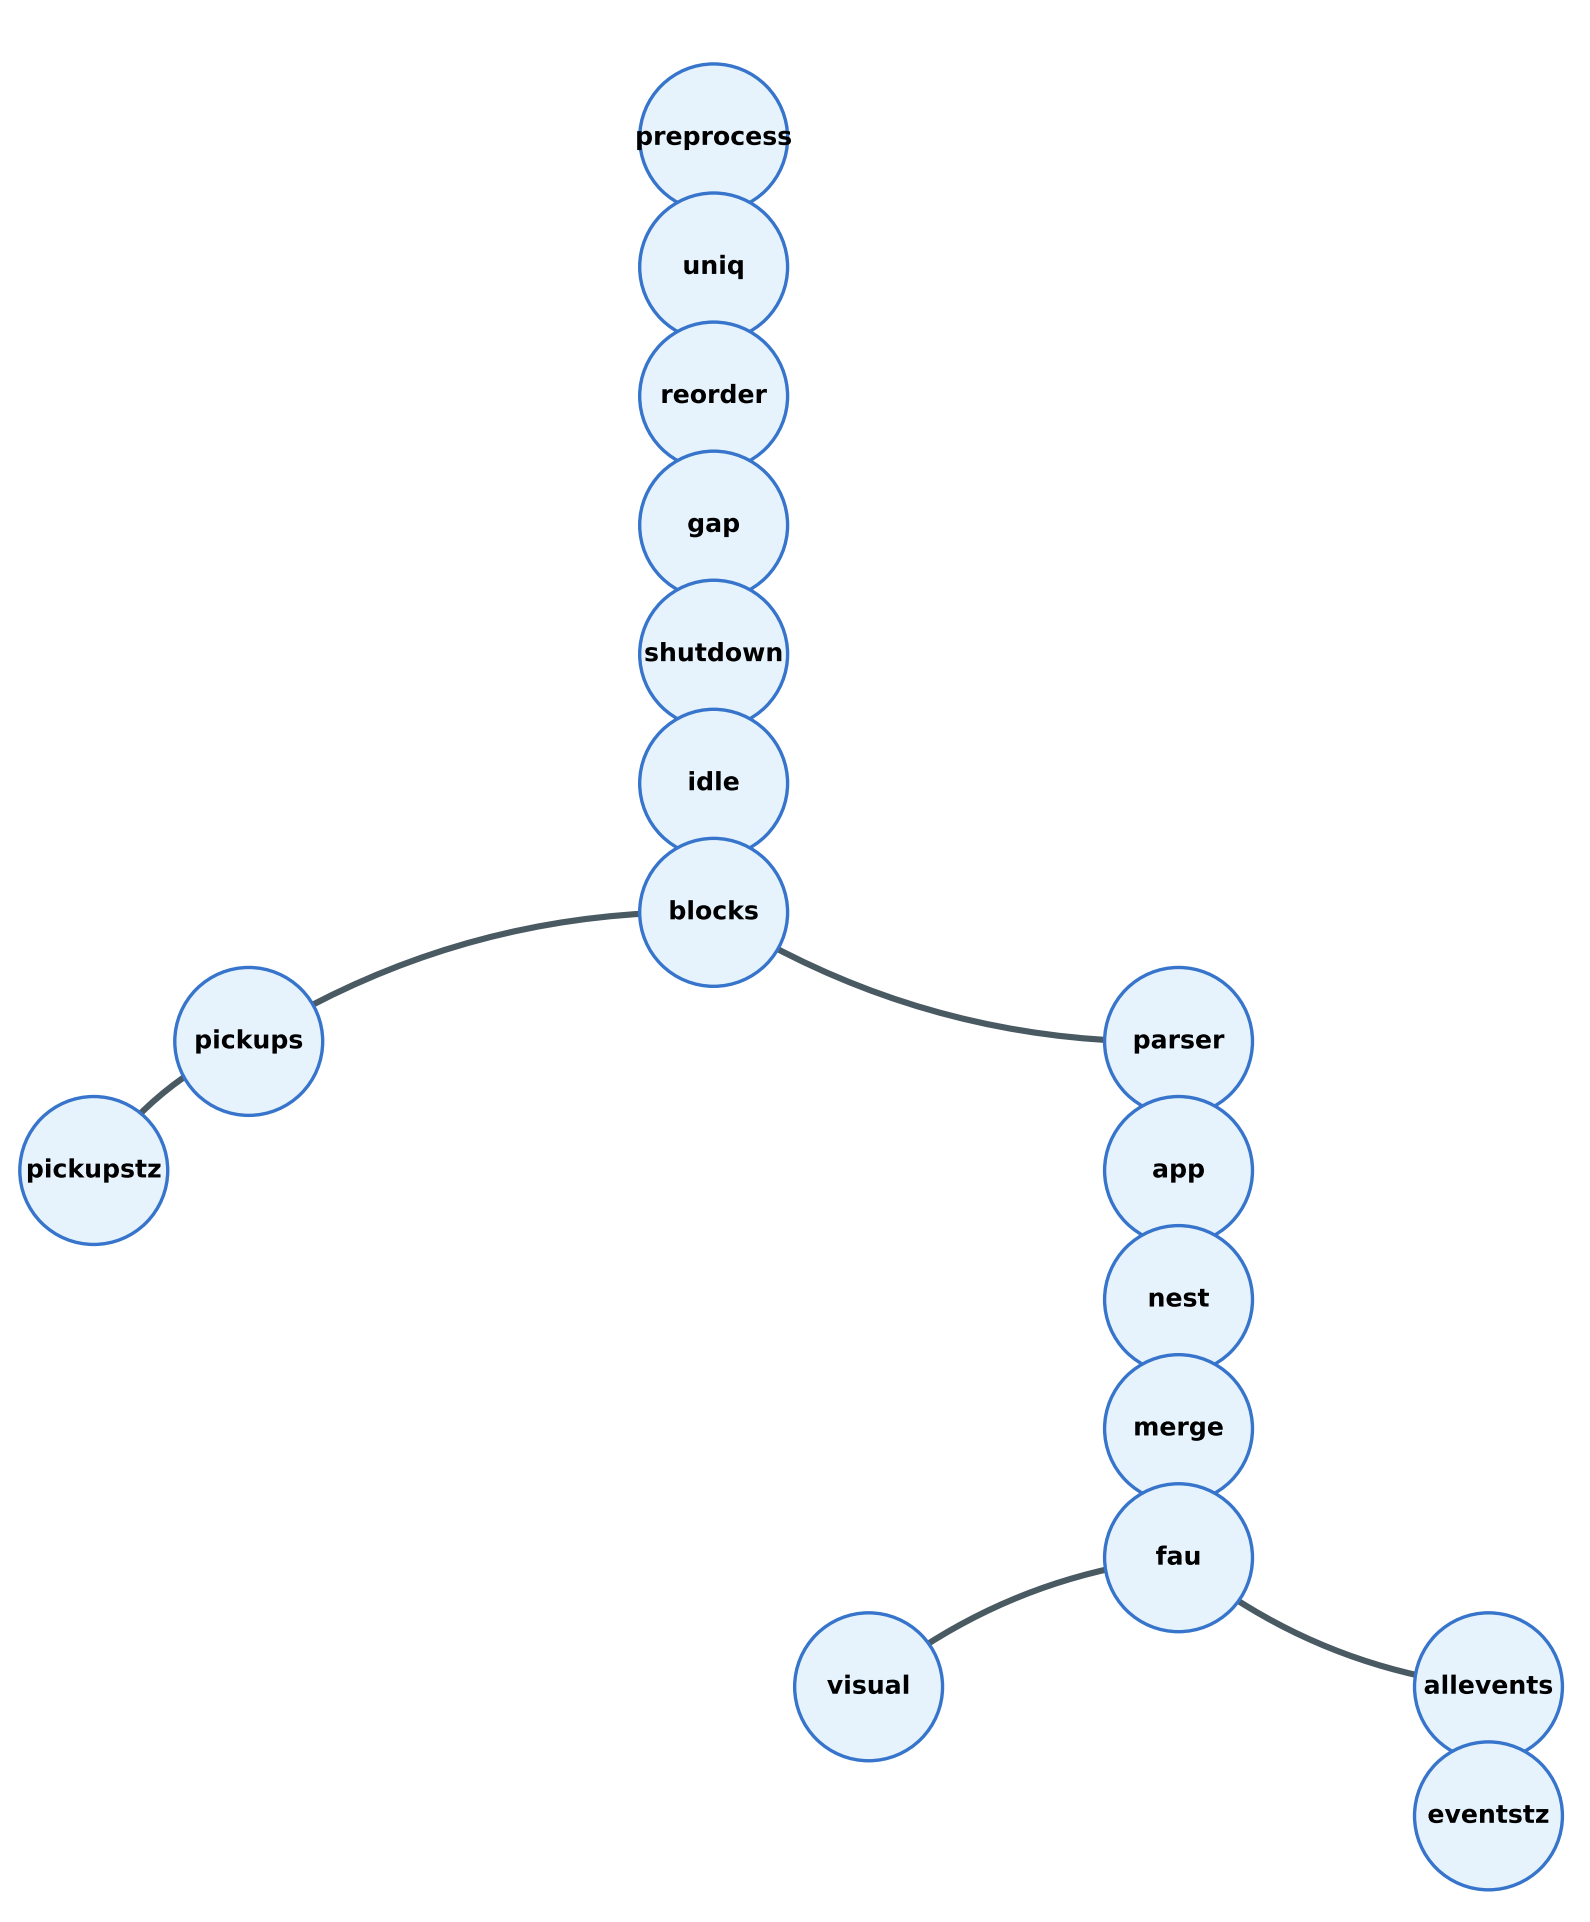
\includegraphics[width=0.55\textwidth]{imgs/units-dependency.png}
  \caption{Dependency of the EYES Processing Units}
  \label{fig:units-dependency}
\end{figure}

\subsection{Phase A: Core Pre-processing}
There are three units in the pre-processing phase: \verb+preprocess, uniq, reorder+.

\begin{enumerate}
\item \verb+preprocess+: This unit does filtering and sorting. 
\begin{itemize}
\item In general, raw Chronicle files do not need to be filtered. However, if a user wants to filter out certain rows based on `interaction type', the scripts provide this functionality. For example, raw files often contain thousands of rows with `Unknown importance: 11'. Filtering out these rows can reduce data size and speed up processing.
\item Sorting is necessary. Since rows in the log file are not always recorded in time-increasing order, we sort the rows by `event timestamp' to maintain a time-increasing order.
\end{itemize}

\item \verb+uniq+: Removes duplicate entries. 

Once the data rows are sorted in the previous unit, \verb+preprocess+, this unit, \verb+uniq+, removes duplicated rows from the data file.

\item \verb+reorder+: Reorder two particular events (Activity Resumed, Activity Paused) when they have identical timestamps. 

This is needed because identical timestamps create ambiguity: according to the timestamp, the two events happen at the same time, but logically one must occur before the other. The \verb+reorder+ unit is designed to place the `Activity Paused' row before the `Activity Resumed' row if both rows have identical timestamps. This resolves the ambiguity. If `Activity Paused' is in fact behind `Activity Resumed' (and thus creates a 0-duration interval between the two events), our \verb+parser+ unit is designed to catch it even if the rows are presented in the wrong order.

For log files collected from old versions of the Android system, we match the tag 'Move to Foreground' and 'Move to Background' to 'Activity Resumed' and 'Activity Paused', respectively.

\end{enumerate}

\subsection{Phase B: Segment Analysis}
The processing units in this phase identify explicit non-active device states and then derive ACTIVE as the remaining time. The states are: ACTIVE, GLANCE, GAP, SHUTDOWN, and IDLE. The SHUTDOWN state indicates that a device is powered off. The IDLE state indicates that a device is in an idle mode in which the screen is off or the device is otherwise not interactive. The GAP state indicates that a device is in either SHUTDOWN or IDLE, but the toolbox cannot determine which state is more likely based on the available data. The GLANCE state indicates that the device screen briefly lights up but does not become unlocked before it turns off again.

In the current design, ACTIVE does not mean that the user is definitely performing meaningful activity. Rather, ACTIVE is the complement of the explicit non-active states:
\[
\texttt{ACTIVE} = \neg(\texttt{SHUTDOWN} \cup \texttt{IDLE} \cup \texttt{GAP} \cup \texttt{GLANCE})
\]
We later combine ACTIVE periods with app activity results to determine whether real user activity occurred.

If a GAP state is present, the user should inspect the logs to determine the likely device state, because in this case the EYES toolbox cannot determine confidently whether the state is SHUTDOWN or IDLE. In general, the user should be alerted if the processing results include too many GAP states.

\begin{enumerate}
\item \verb+gap+: Identifies missing-data periods. This step scans the data rows and compares the timestamps of two consecutive rows. If the timestamp difference is greater than a specified gap threshold, a gap is identified. The gap threshold is configurable, and its default value is 3 hours. If a gap has a duration shorter than 3 hours, it will not be detected by default. A good practice is to process the log data multiple times with different parameters and compare the results to choose the best one.

\item \verb+shutdown+: Detects the periods when the device was powered off. This is done by analyzing the events related to device shutdown/startup in the log file.
\item \verb+idle+: Identifies periods of inactivity. This is done by analyzing the events related to screen interactive/non-interactive and keyguard events in the log file.
\item \verb+glance+: Identifies wake-up periods where the device screen becomes interactive but the device is not unlocked before the screen turns off again. This state is useful because otherwise such periods would be counted as ACTIVE by complement, even though they often do not correspond to real user usage.
\item \verb+blocks+: Categorizes segments and merges them into a single list of blocks in time-increasing order based on the start time of each block.
\item \verb+pickups+: Generates the \emph{pickups} data for the device. The \emph{pickups} data indicates how many times the device was picked up during the observation period. Figure~\ref{fig:pickups} shows the generated pickups data. Rows labeled `ACTIVE' indicate that the device is being used during the interval from `start\_ts' to `end\_ts'.

\begin{figure}[ht]
  \centering
  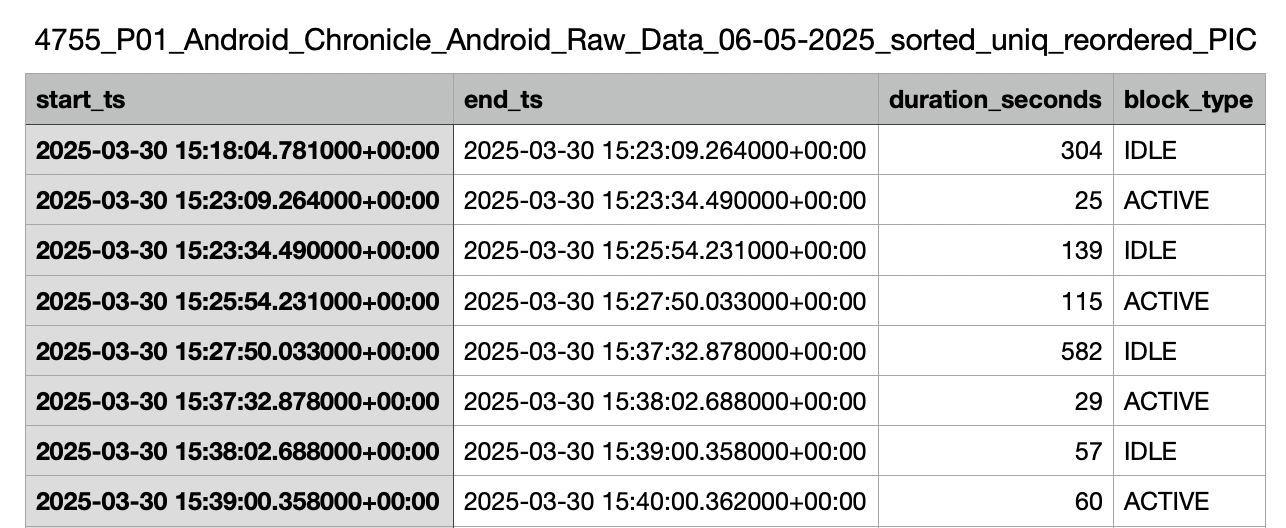
\includegraphics[width=0.75\textwidth]{imgs/pickups-data.png}
  \caption{EYES processing result: Pickups.}
  \label{fig:pickups}
\end{figure}

\end{enumerate}

For each identified period, there is an associated `start time', `end time', and `type'. We call such a period a \textbf{segment}. For a specific segment type, segments are linked together in time-increasing order by their `start time'. Note that a `gap' segment might overlap with a `shutdown' segment.

In the \verb+blocks+ step, we use a more sophisticated algorithm to analyze these segments collectively and identify the state of the device for each period. The outcome of this step is a list of blocks linked in time-increasing order based on the start time of each block. This list captures the device's state changes over time.

\subsubsection{Glance Logic}
The \verb+GLANCE+ state is constructed from the same family of system events used for IDLE analysis, especially:
\begin{itemize}
\item \texttt{SCREEN\_INTERACTIVE} (Unknown importance: 15)
\item \texttt{SCREEN\_NON\_INTERACTIVE} (Unknown importance: 16)
\item \texttt{KEYGUARD\_HIDDEN} (Unknown importance: 18)
\end{itemize}

The logic is:
\begin{enumerate}
\item When a \texttt{Screen Interactive} event occurs at time $t_1$, the toolbox starts a candidate wake episode.
\item The candidate episode is examined until the first decisive event after $t_1$:
\begin{itemize}
\item \texttt{Keyguard Hidden}
\item \texttt{Screen Non-interactive}
\item a SHUTDOWN boundary
\item a GAP boundary
\end{itemize}
\item If the first decisive event is \texttt{Keyguard Hidden}, then the device is treated as unlocked and the interval is \textbf{not} labeled as GLANCE.
\item If \texttt{Screen Non-interactive} occurs at time $t_2$ and no \texttt{Keyguard Hidden} event occurs during the interval $[t_1,t_2]$, then the interval is labeled as \texttt{GLANCE}.
\item If a SHUTDOWN or GAP boundary happens before the screen returns to non-interactive, the candidate wake interval is discarded from GLANCE detection because the wake episode did not close normally.
\end{enumerate}

Therefore, GLANCE captures the behavioral scenario: the screen lights up, but the user never unlocks the device before the screen turns off again.

There is an alternative, more conservative interpretation that could be used in future work. In that alternative design, if a \texttt{Keyguard Hidden} event occurs very shortly \emph{after} \texttt{Screen Non-interactive}, the earlier wake interval might be treated as not meaningful enough to retain as a separate glance. However, this is \textbf{not} the current implementation in the EYES toolbox.

The current implementation only checks whether \texttt{Keyguard Hidden} occurs \emph{within} the candidate wake interval. If the screen becomes non-interactive first, the interval is retained as \texttt{GLANCE}, even if a later unlock-related event is recorded shortly afterward. We keep this implementation for now because it preserves a simple and reproducible interval rule, and because such a glance immediately preceding a later ACTIVE period is not expected to materially affect downstream ACTIVE usage analysis.

\subsection{Phase C: Application \& Event Logic}
\begin{enumerate}
\item \verb+parser+: Parses app activity events to calculate activity-level app usage. The parser respects the logic structure of an app activity. The structure consists of three events: \emph{Activity Resumed}, \emph{Activity Paused}, and \emph{Activity Stopped}.

In general, an app might have multiple activities. For example, when a user interacts with an app that has multiple panels, each of which may correspond to a unique activity, an \emph{Activity Resumed} event will be triggered when the user navigates to a new panel.

If a user launches an App and stays on the first panel $A$ (Activity $A$), then navigates to a new panel $B$ (Activity $B$), multiple events will be triggered in sequence, as illustrated in Figure~\ref{fig:activity-events-order}. Notice that the three events -- Activity Paused (A), Activity Resumed (B), and Activity Stopped (A) -- happen at almost the same time (usually within 1 or 2 seconds). We consider the time duration from Activity Resumed (A) to Activity Stopped (A) as the actual usage time for activity $A$.

\begin{figure}[ht]
  \centering
  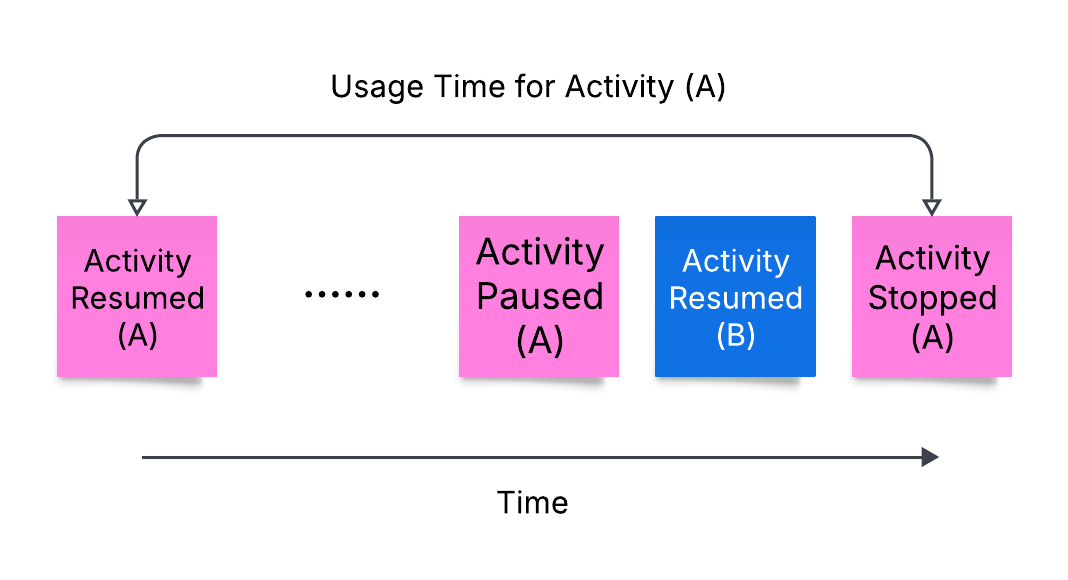
\includegraphics[scale=0.28]{imgs/activity-events-order.png}
  \caption{Android Device Event Ordering for Activity $A$ and Activity $B$.}
  \label{fig:activity-events-order}
\end{figure}


\item \verb+app+: Calculates app-level usage time.

Based on the activity-level usage data processed by the \verb+parser+, in this step we merge the activity usage of the same app to produce app-level usage data. The processed data show all apps and their usage durations, sorted by the resumed time (\emph{Activity Resumed}) of each app.

\begin{figure}[ht]
  \centering
  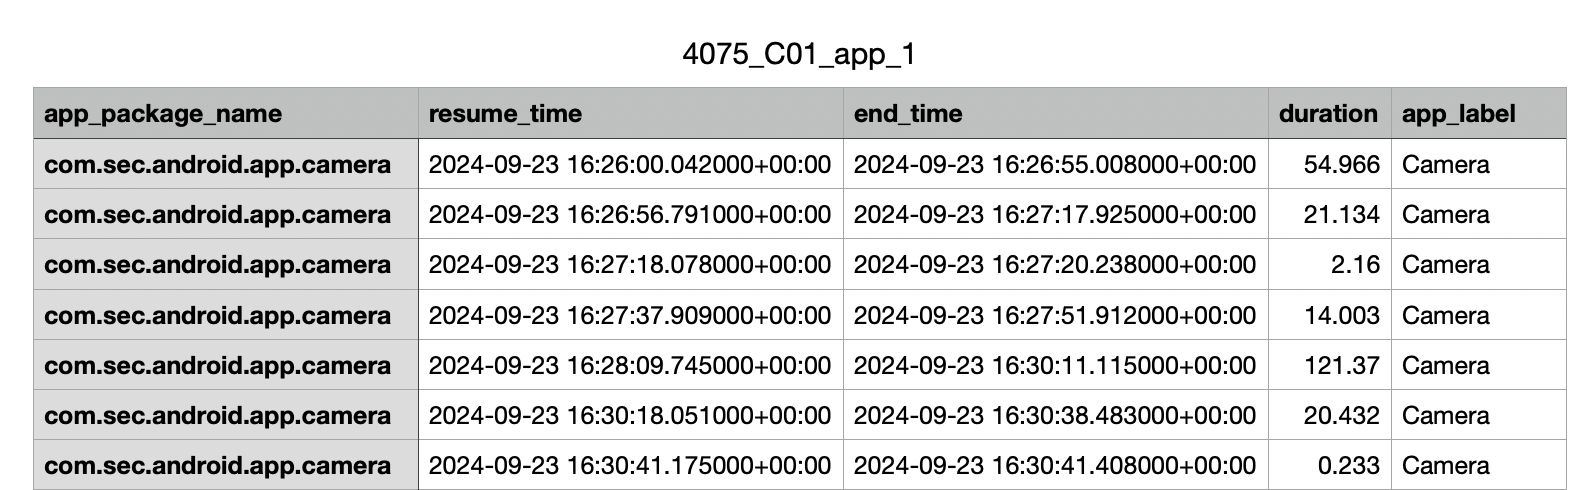
\includegraphics[width=0.75\textwidth]{imgs/app-level-data.png}
  \caption{EYES processing result: App Level Usage Data.}
  \label{fig:app-level-usage}
\end{figure}

\item \verb+nest+: Performs secondary nested analysis on App usage. 

There are scenarios in which a multi-window app (for example, Youtube) is running while another app is also being used by the user. In this case, both apps may have significant overlapping usage time. We still collect the app-level usage and later identify the overlap so that we do not double count usage time. For a given overlapping interval, the processing result will show that one app is the primary usage and the other app is the secondary usage.

\begin{figure}[ht]
  \centering
  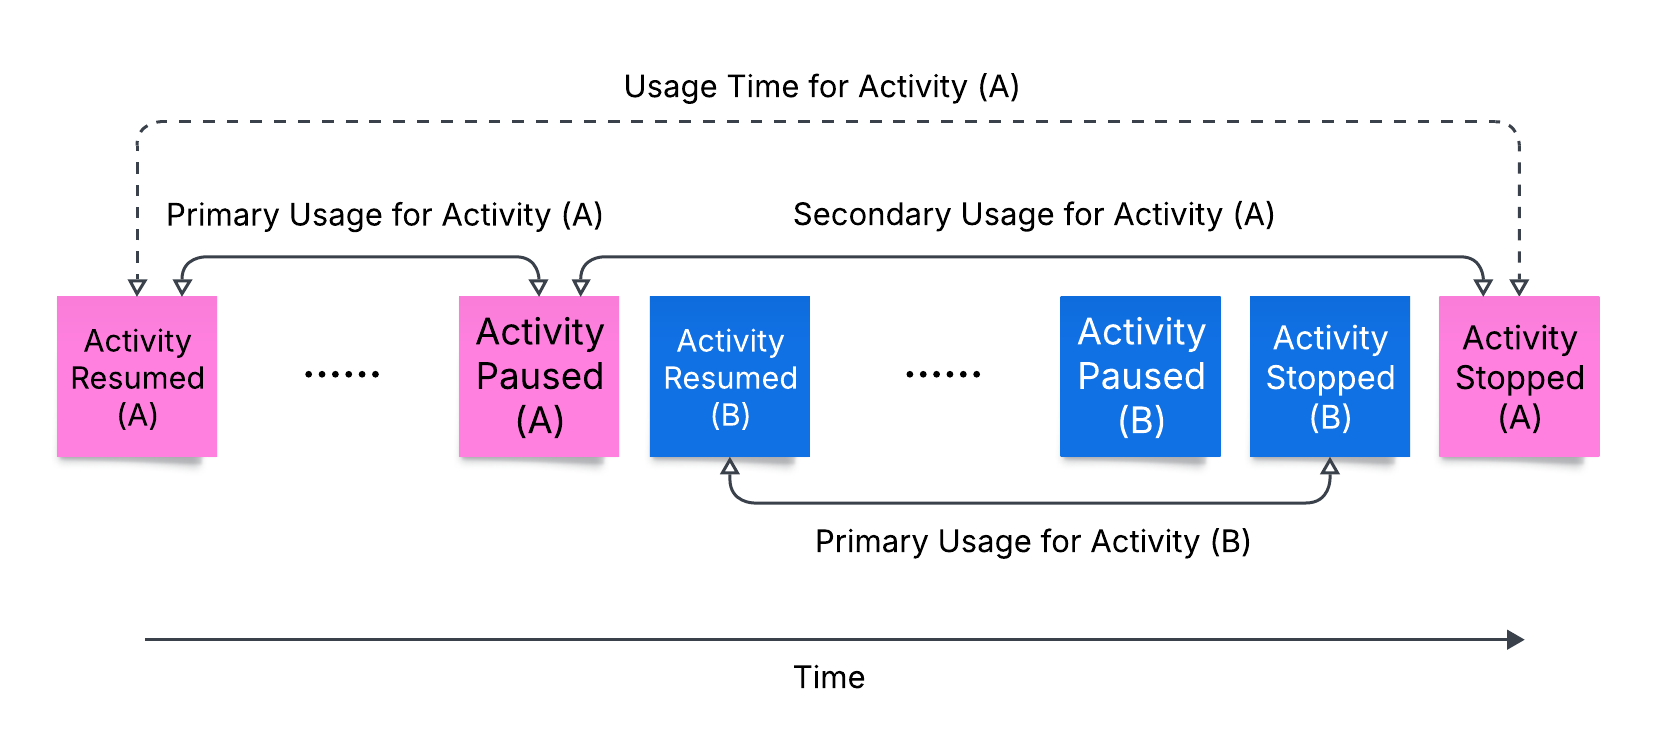
\includegraphics[scale=0.6]{imgs/activity-events-nested.png}
  \caption{Primary Usage vs. Secondary Usage}
  \label{fig:activity-events-nested}
\end{figure}

Figure~\ref{fig:primary-secondary-usage} shows the data generated by the \verb+nest+ unit. There is a `secondary\_duration' column when a given duration is classified as secondary usage for an app.

\begin{figure}[ht]
  \centering
  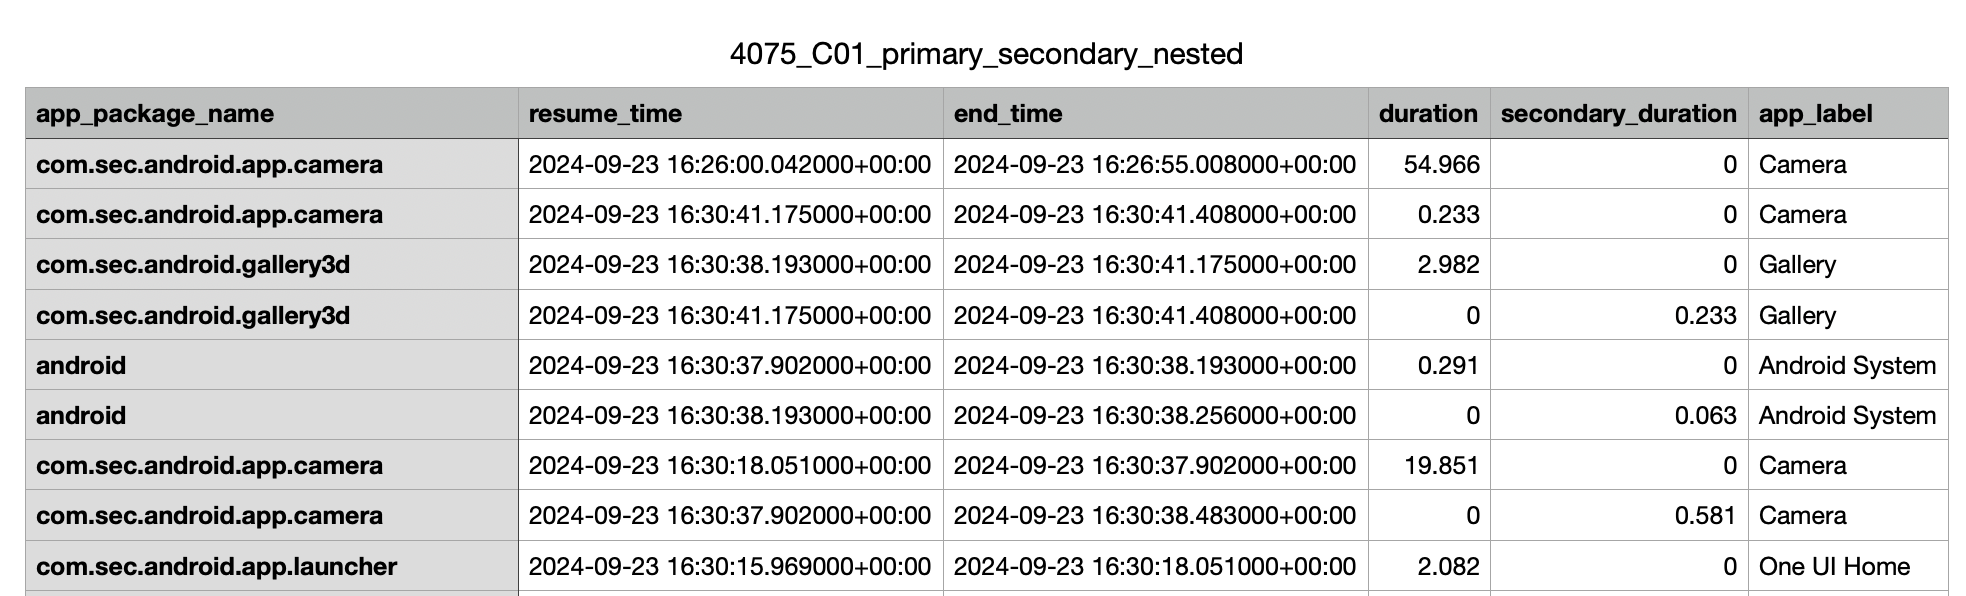
\includegraphics[width=0.75\textwidth]{imgs/primary-secondary-data.png}
  \caption{EYES processing result: Primary and Secondary Usage Data.}
  \label{fig:primary-secondary-usage}
\end{figure}

\item \verb+merge+: Merges device status data with app usage data. This merged dataset has one extra column that labels the device status for each row of app usage data. This extra information is very important for interpreting the usage of a given app. For example, if app usage occurs while the device is in IDLE state, that may indicate that the app was running but the user was not really using it. Figure~\ref{fig:appusage-devicestatus} shows the file format of the merged data.

\begin{figure}[ht]
  \centering
  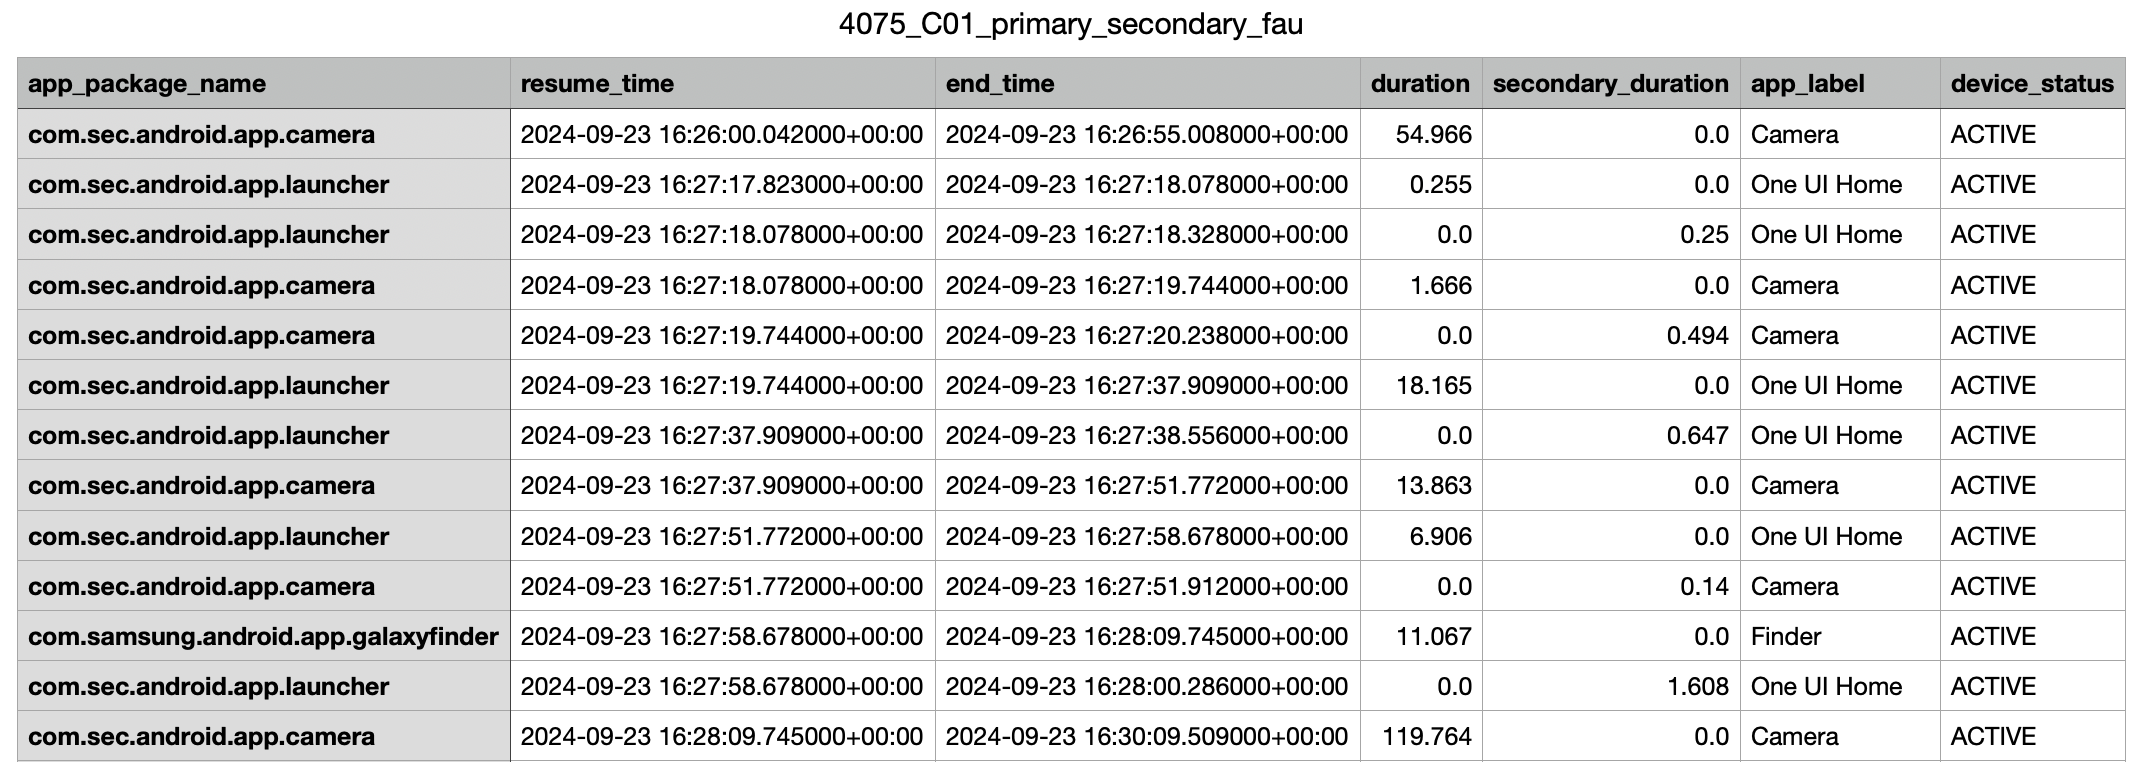
\includegraphics[width=0.75\textwidth]{imgs/appusage-devicestatus-merge-data.png}
  \caption{EYES processing result: App Usage and Device Status.}
  \label{fig:appusage-devicestatus}
\end{figure}

\item \verb+fau+: Calculates ``Final App Usage" (FAU) time, or effective screen time. Once we have the data processed by the \verb+merge+ unit, we use a simple approach to sum all app usage time for a given app under the condition that the device status is `ACTIVE' during the app-usage interval. We refer to this as the FAU time for an app.

If for some reason a researcher wants to sum an app's usage under device status `ACTIVE' or `IDLE', it should be easy to do using the results from the \verb+merge+ unit.
\end{enumerate}

\subsection{Phase D: Final Outputs}
\begin{enumerate}
\item \verb+visual+: Generates a visual display of app usage for a given raw file. This helps researchers understand the data more easily. Figure~\ref{fig:visual} shows an example of app-usage visualization. From the figure, it is easy to get an overview of app usage for each day.

\begin{figure}[ht]
  \centering
  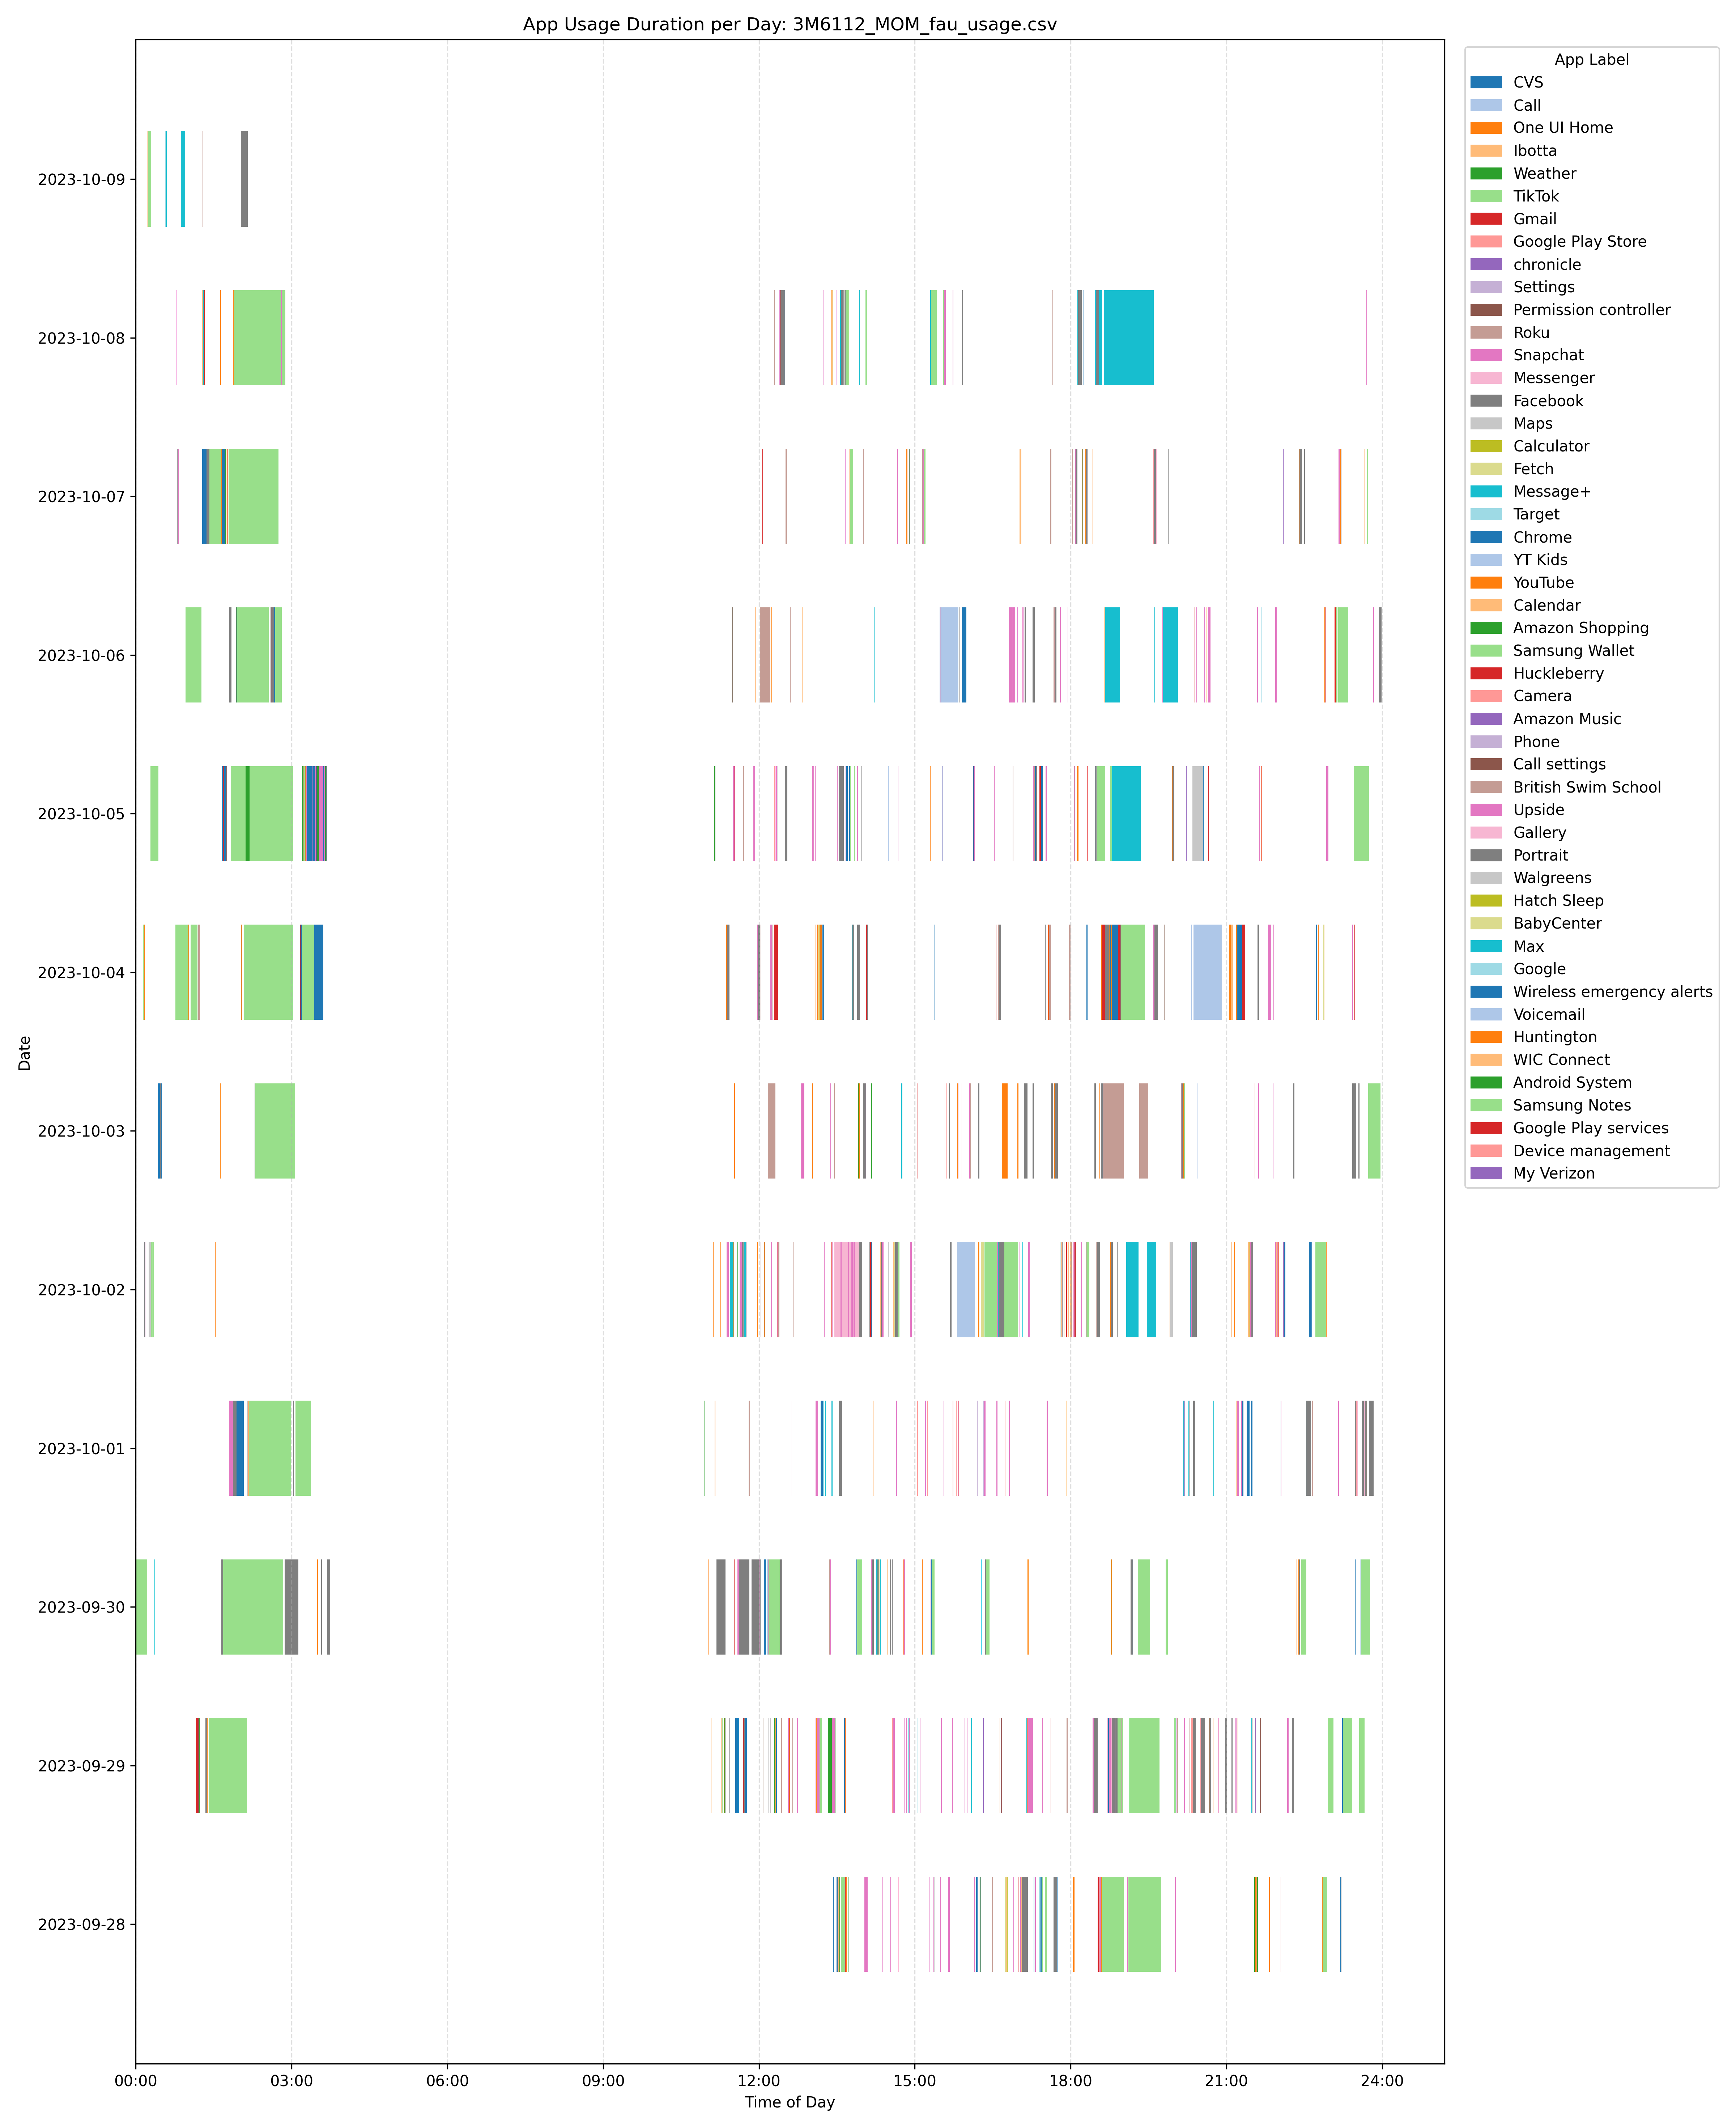
\includegraphics[width=0.65\textwidth]{imgs/3M6112_MOM_fau_usage.png}
  \caption{EYES processing result: Visualization of App Usage.}
  \label{fig:visual}
\end{figure}

\item \verb+allevents+: Compiles a comprehensive list of all detected events and app usage. This output file includes 1) all activity events, 2) all app usage, and 3) device status.
\item \verb+eventstz+: This unit adds timezone information to the data generated by \verb+allevents+. This is the final unit specified in the Makefile. We can use the commands from Table~\ref{tab:commands} to run this unit, and it will trigger all earlier units sequentially. Figure~\ref{fig:all-events-tz} shows the format of the data that integrates all activity events, app usage, and device status.

\begin{figure}[ht]
  \centering
  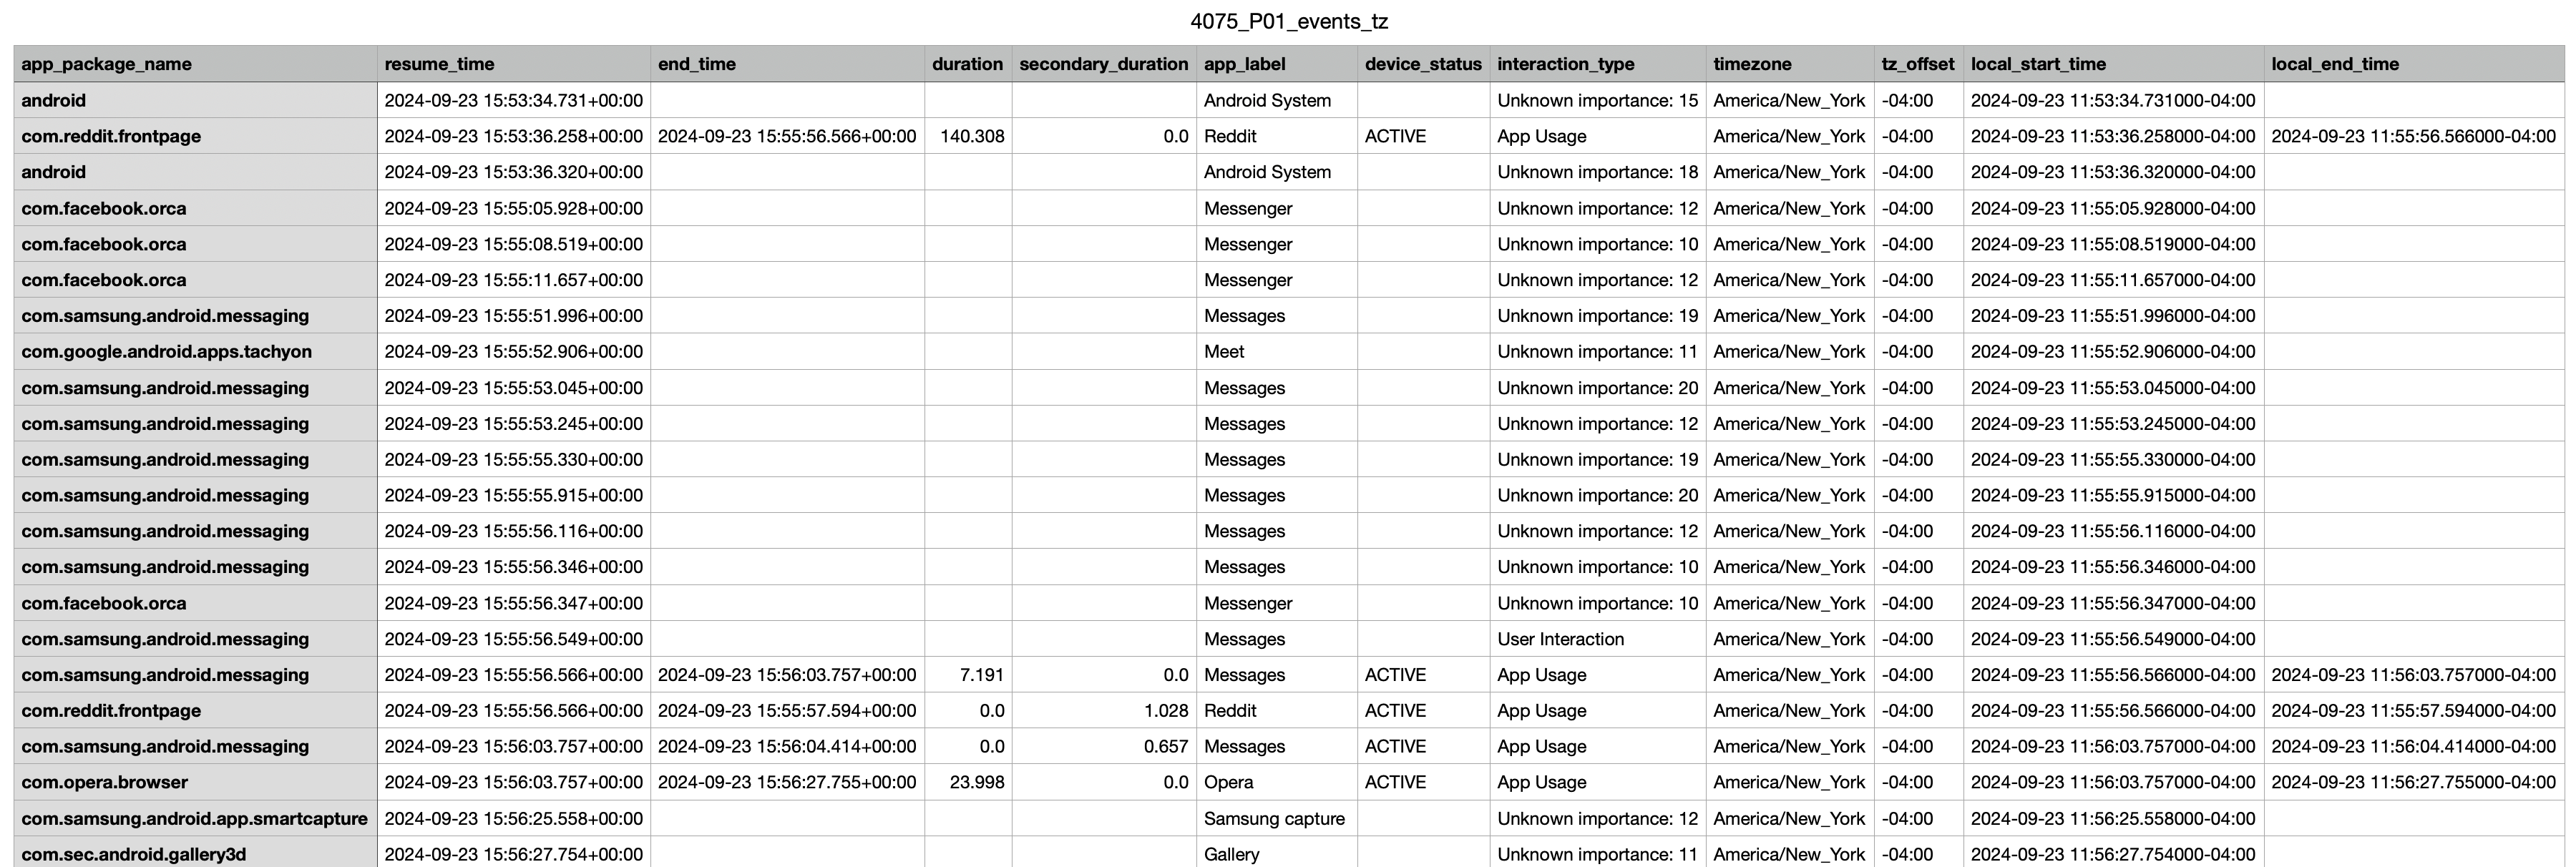
\includegraphics[width=0.75\textwidth]{imgs/allevents-tz-data.png}
  \caption{EYES processing result: All events, App Usage, and Device Status.}
  \label{fig:all-events-tz}
\end{figure}

\end{enumerate}

\section{Usage Commands}
Table~\ref{tab:commands} lists the commands that a researcher can use to run the EYES toolbox scripts. All commands require the data directory to be specified using the \texttt{dir} variable.

\small
\begin{table}
\caption{Major commands to run the EYES toolbox scripts}
\label{tab:commands}
\begin{tabularx}{\textwidth}{|l|>{\raggedright\arraybackslash}p{0.40\textwidth}|>{\raggedright\arraybackslash}X|}
\hline
Full Process & \texttt{make all dir=\path{/path/to/data}} & Run the entire pipeline (Visuals + Pickups) \\
\hline
GUI Launcher & \texttt{make gui} & Launch the EYES desktop GUI. Select a raw-data folder and click \texttt{Go} to run the pipeline. \\
\hline
Clean Up & \texttt{make clean dir=\path{/path/to/data}} & Delete all the processed results (to start over) \\
\hline
Specific Unit & \texttt{make [target] dir=\path{/path/to/data}} & Run up to a specific target (e.g., \texttt{make app}) \\
\hline
The final unit & \texttt{make eventstz dir=\path{/path/to/data}} & Run timezone column adjustment. This will also run all the units ahead sequentially. \\
\hline
\end{tabularx}
\end{table}
\normalsize

\section{Log Events defined in the Android System}
Table~\ref{tab:android_events} shows all the events that are defined in the Android System (in the file \verb+UsageEvents.java+):
\begin{table}
\centering
\caption{Andorid System Events and Numbering}
\label{tab:android_events}
\begin{tabular}{|l|l|}
\hline
Event Name & Unknown importance \# \\
\hline
\hline
ACTIVITY\_RESUMED & 1 \\
        ACTIVITY\_PAUSED & 2 \\
        END\_OF\_DAY & 3 \\
        CONTINUE\_PREVIOUS\_DAY & 4\\
        CONFIGURATION\_CHANGE & 5 \\
        SYSTEM\_INTERACTION & 6 \\
        USER\_INTERACTION & 7 \\
        SHORTCUT\_INVOCATION & 8 \\
        CHOOSER\_ACTION & 9 \\
        NOTIFICATION\_SEEN & 10 \\
        STANDBY\_BUCKET\_CHANGED & 11 \\
        NOTIFICATION\_INTERRUPTION & 12 \\
        SLICE\_PINNED\_PRIV & 13 \\
        SLICE\_PINNED & 14 \\
        SCREEN\_INTERACTIVE & 15 \\
        SCREEN\_NON\_INTERACTIVE & 16 \\
        KEYGUARD\_SHOWN & 17 \\
        KEYGUARD\_HIDDEN & 18 \\
        FOREGROUND\_SERVICE\_START & 19 \\
        FOREGROUND\_SERVICE\_STOP & 20 \\
        CONTINUING\_FOREGROUND\_SERVICE & 21\\
        ROLLOVER\_FOREGROUND\_SERVICE & 22\\
        ACTIVITY\_STOPPED & 23\\
        ACTIVITY\_DESTROYED & 24\\
        FLUSH\_TO\_DISK & 25 \\
        DEVICE\_SHUTDOWN & 26 \\
        DEVICE\_STARTUP & 27 \\
        USER\_UNLOCKED & 28\\
        USER\_STOPPED & 29\\
        LOCUS\_ID\_SET & 30 \\
        APP\_COMPONENT\_USED & 31 \\
        \hline
\end{tabular}
\end{table}
\end{document}
